\documentclass[11pt]{scrartcl}
\usepackage[margin=1in]{geometry}                % See geometry.pdf to learn the layout options. There are lots.
\geometry{letterpaper}                   % ... or a4paper or a5paper or ... 
%\geometry{landscape}                % Activate for for rotated page geometry
\usepackage[parfill]{parskip}    % Activate to begin paragraphs with an empty line rather than an indent
\usepackage[pdftex]{graphicx}
\usepackage{amsmath}
\usepackage{amssymb}
\usepackage{epstopdf}
\usepackage{enumerate}
\usepackage{color}
\usepackage{listings}
\usepackage{booktabs}
\usepackage{xfrac}
\usepackage{float}
\usepackage{amsmath}
\usepackage{sidecap}
\usepackage{palatino}

\newcommand{\noin}{\noindent}    
\newcommand{\logit}{\textrm{logit}} 
\newcommand{\var}{\textrm{Var}}
\newcommand{\cov}{\textrm{Cov}} 
\newcommand{\corr}{\textrm{Corr}} 
\newcommand{\N}{\mathcal{N}}
\newcommand{\NBin}{\textrm{NBin}}
\newcommand{\Bern}{\textrm{Bern}}
\newcommand{\Bin}{\textrm{Bin}}
\newcommand{\Beta}{\textrm{Beta}}
\newcommand{\Gam}{\textrm{Gamma}}
\newcommand{\Expo}{\textrm{Expo}}
\newcommand{\Pois}{\textrm{Pois}}
\newcommand{\Unif}{\textrm{Unif}}
\newcommand{\eq}[1]{\begin{align*}#1\end{align*}}


% \usepackage{natbib, setspace}
\usepackage{setspace}



\DeclareGraphicsRule{.tif}{png}{.png}{`convert #1 `dirname #1`/`basename #1 .tif`.png}


\newcommand{\bs}{\boldsymbol}
\newcommand{\mb}{\mathbf}

\begin{document}

% \onehalfspace


\noindent Computer Science 186 \hfill \today\\
\noindent\makebox[\linewidth]{\rule{6.5in}{2.0pt}}

\begin{center}


{{\LARGE \bf Analysis of Voting Mechanisms}}

\noindent\makebox[\linewidth]{\rule{6.5in}{2.0pt}}

\vspace{3mm}

{\large Yuan Jiang $|$ Lewin Xue} \\
\normalsize yuanjiang@college.harvard.edu $|$ lewinxue@college.harvard.edu \\

\end{center}


\vspace{2mm}

\section{Abstract}

\section{Introduction}

In light of the recent developments for the 2016 Presidential elections, we chose to study various social choice mechanisms and their effectiveness under various circumstances in minimizing loss relative to the socially optimal alternative choice. Social choice mechanisms form a framework for combining individual preferences to reach a collective decision. Different countries around the world employ varying voting mechanisms, with the United States employing simple plurality voting scheme, while many European countries, by proportionally dividing seats based on number of votes, create the need for coalitions to form a majority. These mechanisms are a natural extension of auction design for deciding outcomes where monetary payments are not possible. A large variety of mechanisms have been discussed in the literature, however for the scope of this project, we choose to explore three simple voting mechanisms that are used universally in elections: plurality, majority with a top-2 runoff, and Borda vote; as well as a recently introduced ``Democracy 2.1'' voting mechanism. We believe each of these mechanisms have the opportunity to be applied in real elections based on the simplicity of their designs.\\

Various social choice designs result in different properties that we find attractive in different circumstances. Three out of the four voting mechanisms we chose to study are therefore positional voting rules, which satisfy the qualities of neutrality, anonymity, weak monotonicity, non-constancy, consistency, and continuity that we believe are necessary for any successful election mechanism. While the top-2 runoff isn't a direct positional voting mechanism, we believe that by first performing majority voting, and then performing another majority vote on the top 2 candidates if there is no clear winner also forms a positional voting system. In doing so we sacrifice the Condorcet criterion that holds for pairwise majority voting.\\

Furthermore we choose to ignore voter strategies outside of truthful reporting in our simulations of various voting mechanisms. We do note that for a small number of voters, positional voting schemes can easily have many beneficial deviations for each specific agent. However as we wish to base our studies off of a presidential election, our simulations will have many more agents (100) and the coalition size required for such manipulations to be successful (size $>\sqrt{n}$) would be difficult to obtain in the real world. Furthermore outside of the straight plurality voting mechanism, finding beneficial deviations of the other positional voting scheme is not tractable. Based on these two difficulties in applying deviations in a general election, we deem strategic, non-truthful voting to be beyond the scope of our discussion.\\

Finally to better simulate the irrationality of voters in real life, we decided to add noise to our agent's preferences, which were drawn from predetermined distributions. We believe that under practical conditions, one cannot expect fully rational or even fully self-aware agents, and so noise would better reproduce challenges faced in designing and applicable voting mechanism. In doing so, we wish to study how this noise would affect the robustness of various voting schemes and whether under specific schemes the noise would cancel out or reinforce itself to create outcomes that were on average farther away from the socially optimal outcome.\\

Our simulations cover the four voting mechanisms over 3 prior distributions for preferences (uniform, normal, and tight), and over noisy versus noiseless. We hope to determine the best mechanism out of the four for large-scale general elections that minimizes the loss of social utility.

\vspace{2mm}

\section{Methodology}

\subsection{Plurality Voting}

Plurality voting is perhaps one of the most common and simple voting mechanisms that exists. Under this voting mechanism, the candidate with the most number of votes wins. Plurality voting is often known for being a poor mechanism in terms of maximizing collectional social welfare in tight election where two or more candidates are very popular among the voting population. Most famously, the shortcomings of the plurality election were exposed in the 1860 U.S. Presidential election in which the victor, Abraham Lincoln, secured 39.8\% of the popular vote, one of the lowest popular vote percentages in the history of U.S. presidential elections. His immediate successor Stephen Douglas secured 29.5\% of the popular vote. At the time, there was great unrest between the northern and southern states, and Lincoln was able to secure his candidacy, without carrying a single southern state, which would later fuel the start of the American Civil War.\\

Our algorithm broke ties similarly to the majority runoff elections that will be detailed below.

\subsection{Majority Voting}

Majority voting requires a strict majority of voters to select a candidate for said candidate to become elected. As traditionally such majorities are difficult to achieve, we decide to hold a runoff election between the top-2 candidates should there not be a strict majority. In this case top-2 refers to the candidates that have either the most or second most number of votes. If there is a tie for second place, all candidates with the second most number of votes will be cast into the runoff (note if there is a tie for first place, only the first place candidates are eligible for the runoff). In the runoff election a strict majority is once again required to win.\\

Our motivation for choosing the runoff model rather than performing the pairwise majority model as specified in Chapter 15 of the textbook was to maintain simplicity and a positional scoring rule. We wanted to compare different voting mechanisms along the same set of scoring rules, and using a top-2 runoff appeared to be the fairest and that best simulated an outcome that would occur in the real world. Furthermore this runoff model generalizes across the four studied voting mechanisms as a feasable runoff decision maker with the same spirit for only two candidates.

\subsection{Borda Count}

The Borda Count method is a single-winner election method in which voters rank $n$ candidate in order of preference from 1 (most preferred) to $n$ (least preferred). Candidates are then assigned a number of points inversely corresponding to their rank (i.e. candidates with lower rankings, who are more preferred, get more points), and the winner is determined by choosing the candidate with the highest number of points. In the event of a tie, we resolved it with the same runoff election as in the majority election. The Borda count often elects widely accepted candidates, rather than the candidate preferred by the majority, and is thus often labeled as a consensus-based voting system.\\

The Borda Count is currently used in many real elections such as the presidential election in Kiribati, the Parliamentary election in Nauru, as well as many non-political elections by private organizations. \\

For the purposes of our simulations, in an election with $n$ candidates, a candidate that receives an $i$-th ranking receives $n-i+ 1$ points (e.g. in an election with 10 candidates, a candidate who is ranked first receives 10 points). 

\subsection{Democracy 2.1} 

Democracy 2.1 is a newly proposed voting mechanism by Czech anti-corruption activist Karel Janecek that is aimed toward reducing extremism voting. It is a blend of traditional majority voting and disapproval voting, in which each voter is given two "positive" votes and one "negative" vote. The two equally-weighted positive votes are cast for the top two preferred candidates while the negative vote is cast for the least preferred candidate, and each "negative" vote can be thought of as incurring a penalty.

Each vote counts either as $+1$ for the positive vote, or $-1$ for the negative vote. Ties are still broken using the majority runoff model, as in races with only two candidates, the positive and negative votes "cancel" for the less prefered candidate, breaking the race down to a majority race.

\subsection{Simulations, Preferences and Noise}

Simulations were run with 100 voters, 5 candidates, and 1000 iterations. For each iteration, the same candidate preferences were preserved and all 4 voting mechanisms were simulated. Utility loss was calculated as:

\[\textrm{utility loss} = \textrm{optimal candidate utility} - \textrm{winner utility}\]

We create 100 voters with different preferences over the 10 available candidates. We have 2 different distributions from which the preferences are created. First there is a uniform (0,1) distribution over all of the candidates. Second we simulated a with candidate preferences being drawn sampled from a standard uniform distribution and a shifting Normal distribution. For candidate $i$, the preference was sampled from a $N(\sqrt(i), (i + 1)^2)$ distribution -- thus, candidates with higher ID numbers were slightly more preferred by the general population. We believe that candidates that are more preferred are more likely to have disagreement over their value. Based on the continual nature of these distributions, we are able to ensure that every voter has strict preferences over the candidates for computational simplicity.

\textbf{\^ CHANGE ABOVE}


In a practical sense, ten candidates appears perfectly rational to have as the total number of candidates. However in most cases the race will simply be between the two leading parties in a "tight" election. To simulate this tightness we continue to create preferences as above; next we replace the preferences for candidates 1 and 2 with an exponential prior with $\Expo(\lambda = 2)$. Over 100 voters, one of candidate 1 or 2 now is most likely to be the socially optimal candidate.

Finally we discussed in the introduction our desire to add noise to the voter preferences to capture voter irrationality and uncertainty. After creating the preferences as described above, we then add standard normal noise to each of the preferences over all voters. We explore how this noise negatively affects outcomes and each mechanism's robustness in response to this noise.

Thus we study eight different total preference distributions. Uniform, tight or not tight, and noisy or noiseless. And normal, tight or not tight, and noisy or noiseless. We run 1000 iterations, where each iteration generates a set of voters and then runs all eight election types.

\section{Results and Discussion}

In many of our simulations, we found that Borda Count would result in the lowest average utility loss. This is reasonable since first, widely accepted candidates are often elected and second, more information (voters reveal entire preference) is being used when it comes to determining the final winner.  

Below, we expore the results of the simulations we ran. We begin by looking into non-tight elections under both the uniform prior as well as the normal priors discussed in the methodology.

\subsection{Uniform "Loose" Elections}
\begin{figure}[H]\center
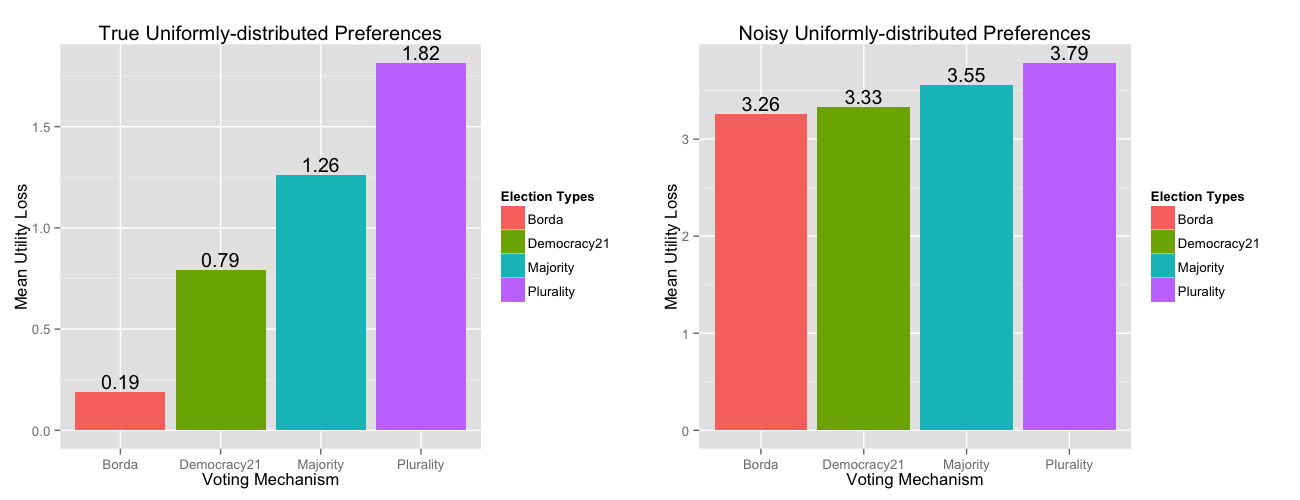
\includegraphics[scale=0.38]{uniform.png}
\caption{Bar graph of average utility losses for each election under uniformally distributed preferences and truthful reporting and noisy reporting}
\end{figure}

<<<<<<< HEAD
From the visualization above, we observe that in a truthful election, Borda Count does noticeably better than the other mechanisms while plurality incurs the highest loss (for reason discussed previously). However, when noise is added to each voter's preference, we see that the utility loss of each election increases and the differences between each mechanism are drastically decreased. 
=======
Figure 1 shows the success of Borda count over the other simulated voting mechanisms. By the central limit theorem the total social utility follows a normal distribution. The mean of the distribution is simply the sum of the expected values to give 50. The standard deviation can be found by $n^2 * \sigma^2/n$, where $\sigma^2$ is the variance of the uniform distribution. This gives us a standard deviation in the sum of $2.88$.

Using order statistics, the expected utility of the best candidate should be $50 + 1.3*2.88 = 53.74$. Note we use 1.3 because it corresponds to 91\%, or where we would expect the best candidate to fall. Empirically we found this to be close to the social utility of the optimal candidate under uniform priors.

Borda count averages a loss of only .19, where the average social utility per candidate is 53.74. Thus we lose out only 6\% of a standard deviation from the optimal candidate in general. Assuming infinite candidates who were distributed along this normal distribution, this moves us from the candidate in the 91st percentile to a candidate in the 89th percentile on average. The limited number of candidates means this loss isn't very noticeable. In fact looking at the second best candidate, we would expect him to fall on the 82nd percentile. Thus we note that the average loss from Borda count is extremely small relative to the optimal candidate, and thus in general we tend to choose the best candidate among the ten selections.

Democracy 2.1 fares slightly worse in choosing a candidate that is on average 0.79 worse than the optimal candidate moves us $.79/2.88 = .274$ standard deviations away from the optimal solution. In this case we have regressed from choosing a candidate in the 91st percentile to a candidate in the 86th percentile. Again we tend to be choosing either the socially optimal candidate or the 2nd best option.

Plurality voting performs the worst under the uniform preference order, having an average loss of 1.82. This moves us $1.82/2.88 = .63$ standard deviations away from the optimal candidate. We are now choosing approximately the 75th percentile candidate. Thus we are on average choosing a candidate worse than the 2nd best candidate using plurality voting. There is a much higher variation on the level of candidate that ends up being elected by the plurality mechanism. This demonstrates some of the dangers of plurality voting.

These voting trends are unsurprising for the uniform prior preferences. Additional information appears to be the best determinant in selecting the optimal candidate. Borda count forces the voters to reveal their entire preference order, Democracy 2.1 the top 2 and bottom choice, and plurality and majority only the top choice. However because of the tendency for runoffs in majority voting, there frequently is more information revealed in the form of choosing again over a limited set of candidates. Information revealed by each voter appears to correspond directly with an improved ability of the mechanism to choose the optimal candidate as voters are voting truthfully.\\
>>>>>>> 2994a4c945f55efb1c3f6eec48ec03f3d6134546

Once noise is added into the system all of our mechanisms perform significantly worse than before. In fact even the best performing Borda count still averages a loss of 3.26, indicating the average chosen candidate is only $.17$ standard deviations better than the average candidate. We are thus on average picking the 4th best candidate. For the three other mechanisms, we perform at a level that can be seen equivalent to randomly choosing a candidate as the victor.

In this case, the noise added in the form of a standard normal heavily affected the perceived preferences of the voting mechanism. Because of the relatively small differences in preferences under the uniform mechanism, the standard normal completely overpowers the original true preferences. Thus as expected, voting mechanisms do as well as random selection when the voters themselves have no idea as to their real preferences and only know their noisy, "irrational" ones.


\subsection{Normal "Loose" Elections}
\begin{figure}[H]\center
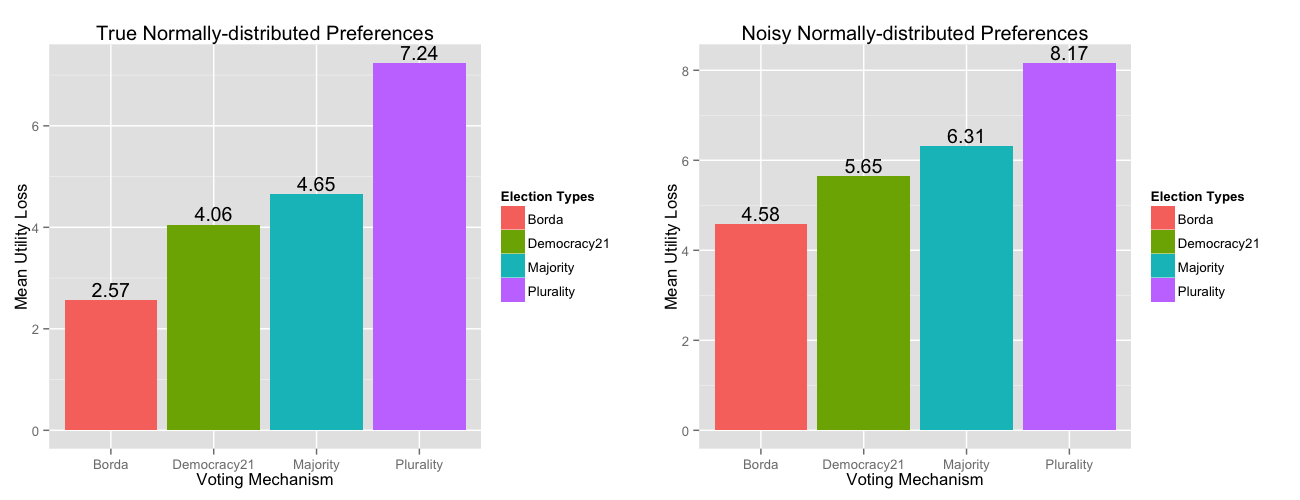
\includegraphics[scale=0.38]{normal.png}
\caption{Bar graph of average utility losses for each election under normally distributed preferences and truthful reporting.}
\end{figure}
Here, we observe that with Normally distributed preferences...

Figure 2 shows the results of creating a preference order among the candidates, where candidates with higher ids are more preferred by the voters on average. Again we can study the average loss and see how various mechanisms perform. In this case because we have predetermined the "best" candidate, we know that the average optimal utility will be 100, while the second best utility will be 90. However the on average more preferred candidates are subject to more variance, which makes the ability of the voting mechanism to respond to this variance interesting.

Again, unsurprisingly Borda vote performs the best followed by Democracy 2.1, majority and finally plurality. Yet once these candidates have more separating them, all of the election mechanisms tend to choose either the best or at the very least the 2nd best option. Borda count has the least average loss at 2.57 and tends to pick the socially optimal agent. Because agents are no longer all selected along the same distribution it isn't possible to remark about the "percentile" as we did for uniformly distributed preferences. Democracy 2.1 and Majority both tended to choose the socially optimal agent given their average utility losses of $<5$. Plurality voting stood as the only mechanism that did not choose the socially optimal candidate the majority of the time.

This can be understood as information release similar to the truthful uniform preferences. The mechanism that releases the most information from the voter will produce the best result. In particular we note the effect of variance in each of the voter's preference for a particular candidate as fairly high relative to the mean, and higher for on average more preferred voters. In that case plurality can easily create cases where the candidate that is socially optimal loses out because voters split their votes among a larger set of candidates. This is also possible under the other three voting mechanisms, but is less likely.

The addition of standard normal noise to each of the voter's preferences again cause the average utility loss to rise for each of the four studied mechanisms. This is not surprising. Unlike the prior exercise where standard normal noise was added to the uniform distribution, here the noise is not strong enough to completely cancel out the signal.

What is interesting is how much worse each mechanism does after introducing noise. We note that Borda count does significantly worse around 2 utils, compared to plurality which only does only 0.93 utils worse. Majority and Democracy 2.1 fall in between these two. This occurs because the addition of noise becomes compounded in each additional candidate preference that is significant for the voting mechanism. Thus mechanisms that require more voter information, are more sensitive to the addition of noise than those that require less information. However heavily information revealing mechanisms (Borda) still perform better than low information revealing mechanisms (plurality) on maximizing overall utility, performing relatively worse to the non-noisy baseline.


\subsection{Uniform Tight Elections}

\begin{figure}[H]\center
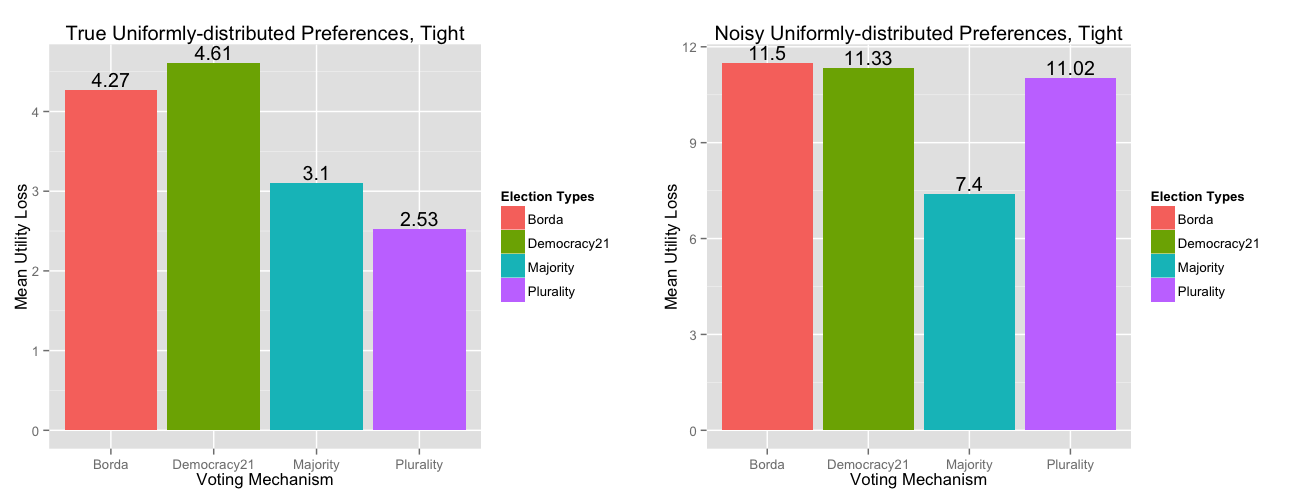
\includegraphics[scale=0.38]{uniform_tight.png}
\caption{Bar graph of average utility losses for each election under normally distributed preferences and truthful reporting.}
\end{figure}

Figure 3 shows the relative performance of the 4 voting mechanisms in the scenario where 2 candidates should be strongly preferred compared to the other 8. The introduction of tight election voting with a uniform (0,1) prior essentially ensures that the socially optimal candidate is either candidate 1 or candidate 2. While sampling over the exponential distribution with mean 2 still allows other candidates a chance to be the most preferred for a specific voter, most voters will prefer one of the "tight" candidates.

The exponential distribution lends itself well to the central limit theorem, and we note that with lambda=2, the average tight candidate will have a social utility distributed over a normal distribution with mean 200, standard deviation 20. Using the same analysis as with the loose uniform elections, we note the utility of the best candidate should be the $66$th percentile of the normal distribution. This is .4 standard deviations above the mean, resulting in the best candidate having an average utility of 208, and the 2nd best candidate having a utility of 192.

Given the average loss for non-noisy voting is always less than 5, we can conclude that every voting mechanism tends to select the socially optimal candidate above 50\% of the time. Given that the average for the second tight candidate is so much higher than the other candidates, we can assume that only these two candidates will be chosen.

In the tight election plurality actually performs the best averaging only 2.53 utils of loss, with the majority voting mechanism closely following, and Borda and Democracy 2.1 trailing behind. Surprisingly unlike the loose elections discussed in section 4.1 and 4.2, additional information release appears to be a negative in elections primarily between two candidates. However the difference can be explained by the distribution of how the tight candidates are chosen.

In particular consider Democracy 2.1. Even if a candidate strongly prefers candidate 2 to candidate 1, he still most likely prefers these two candidates to anyone else in the field and thus weights them equally.  Because of how the exponential distribution is structured, voters can be in the "fat tail" or have strong positive utility from a certain candidate being elected, yet have essentially no say on the outcome of the election as he voted for both of the top two candidates. The deciding factor then comes not from this voter with strong preferences, but rather from the voter who prefers a candidate from the field to either one or both of the two tight candidates, say candidate $x$. These users will actually see minimal difference between the tight candidate who did not receive the vote and candidate $x$ just by the nature of the limited upside of the uniform distribution. Thus Democracy 2.1 overweighs the significance of those with minimal gains in utility, while underweighting those that may have very large gains in utility.

Borda vote does something similar, only allowing it to be likely that the tight candidate still receives a relatively high position. However the determining factor will still be more marked if a voter prefers a non-tight candidate to a tight candidate. In this case plurality and majority actually are the best mechanisms to ensure that those with strong positive opinions for a certain candidate are able to best make their preferences known. By limiting votes to only one candidate, the mechanism puts more weight on the possibility for heavy positive preference, and allows voters to directly vote between the two tight candidates, rather than placing the emphasis on the others.


\textbf{noise needs to be redone}


\subsection{Normal Tight Elections}

\begin{figure}[H]\center
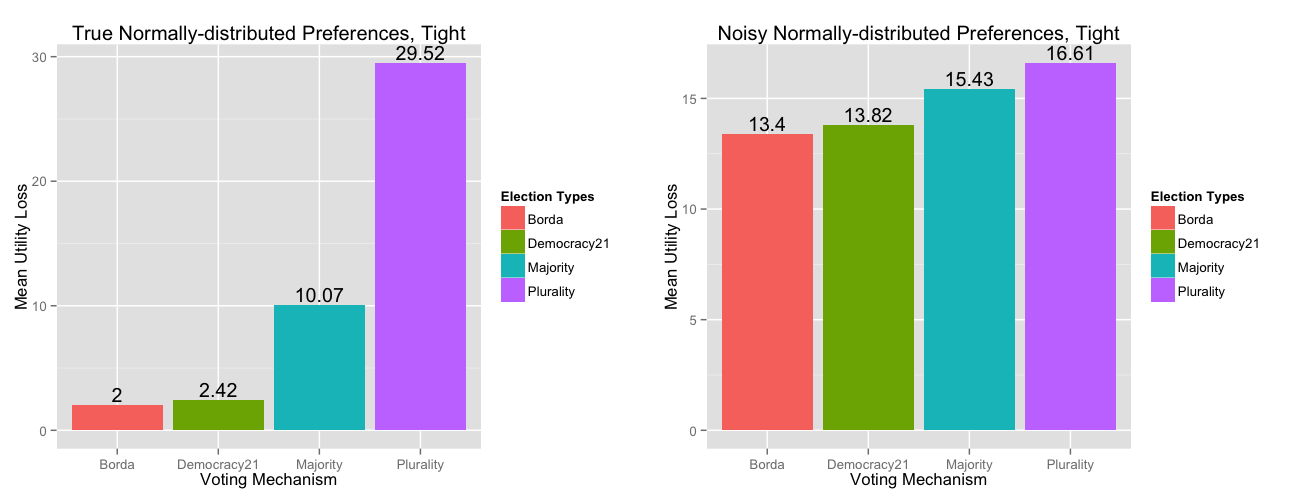
\includegraphics[scale=0.38]{normal_tight.png}
\caption{Bar graph of average utility losses for each election under normally distributed preferences and truthful reporting.}
\end{figure}

\textbf{this needs to be redone}


\section{Final Remarks}

Borda count, while successful may be less so as you require candidates to have an idea about their preferences over ALL candidates

\end{document}




